\documentclass[11pt]{article}
\usepackage{amsmath}
\usepackage{pdfpages}
\usepackage{microtype}
\usepackage{algorithm}
\usepackage[noend]{algpseudocode}
\usepackage{setspace}
\usepackage{mathtools}
\DeclarePairedDelimiter\ceil{\lceil}{\rceil}
\DeclarePairedDelimiter\floor{\lfloor}{\rfloor}
\usepackage{hyperref}
\usepackage{listings}
\usepackage{float}
\usepackage{amssymb}
\usepackage{physics}
\usepackage[margin=0.75in]{geometry}
\usepackage{multicol}
\usepackage{titlesec}
\usepackage{titling}
\usepackage{graphicx}
\lstdefinestyle{mystyle}{
	basicstyle=\ttfamily\footnotesize,
	breakatwhitespace=false,         
	breaklines=true,                 
	captionpos=b,                    
	keepspaces=true,                 
	numbers=left,                    
	numbersep=5pt,                  
	showspaces=false,                
	showstringspaces=false,
	showtabs=false,                  
	tabsize=2
}
\lstset{style=mystyle}
\setcounter{tocdepth}{3}
\usepackage[nottoc,notlot,notlof]{tocbibind}
\title{\Huge{ECE470:Network Client-Sever Programming}\\\LARGE{Project 1: Part 1}}
\author{Aaron Jesus Valdes}
\begin{document}
	\maketitle
	\clearpage
	\tableofcontents
	\onehalfspacing
	\clearpage
	\section{Project Description}
	Designing a smart home remote access system which follows the Network/Client architecture. This system allows the user to control certain devices from their home such lights, alarm, and locks from a remote location.
	\section{Specifications}
		\begin{itemize}
			\item Supports smart lights
				\begin{itemize}
					\item Can turn on and off lights
					\item Can change the color and brightness of lights
					\item Groups lights into rooms
				\end{itemize}
			\item Supports alarm system
				\begin{itemize}
					\item Can arm and disarm the alarm
					\item Can have more than one alarm system
					\item Can store 4 digit pin per alarm 
				\end{itemize}
			\item Supports Electronic Locks
				\begin{itemize}
					\item Can open and lock the locks
					\item Can have more than 4 locks
					\item Can store a 5 digit pin per lock
				\end{itemize}
			\item Supports more devices
				\begin{itemize}
					\item Can control the thermostat
						\subitem Turn on or off heat/cold
						\subitem Set temperature
					\item Can check the security cameras
						\subitem Can store the video from a security camera
					\item Can control blinds and drapes
						\subitem Opens and closes the blinds
				\end{itemize}
		\end{itemize}
	\section{Assumptions}
		\begin{itemize}
			\item We are only working with a single house
			\item There are multiple rooms in the house
			\item Each room has multiple lights
			\item There is only one alarm
			\item There are at least 4 locks
			\item One user at a time can connect
			\item The server is in the home
			\item The server can be accessed both inside and outside of the house
			\item The user needs to check and alter status of the devices
			\item The method of communication is
			\item The server must be protected by having a login page
		\end{itemize}
	\section{Initial Design}
		\subsection*{Data Model}
			\begin{figure}[H]
				\centering
				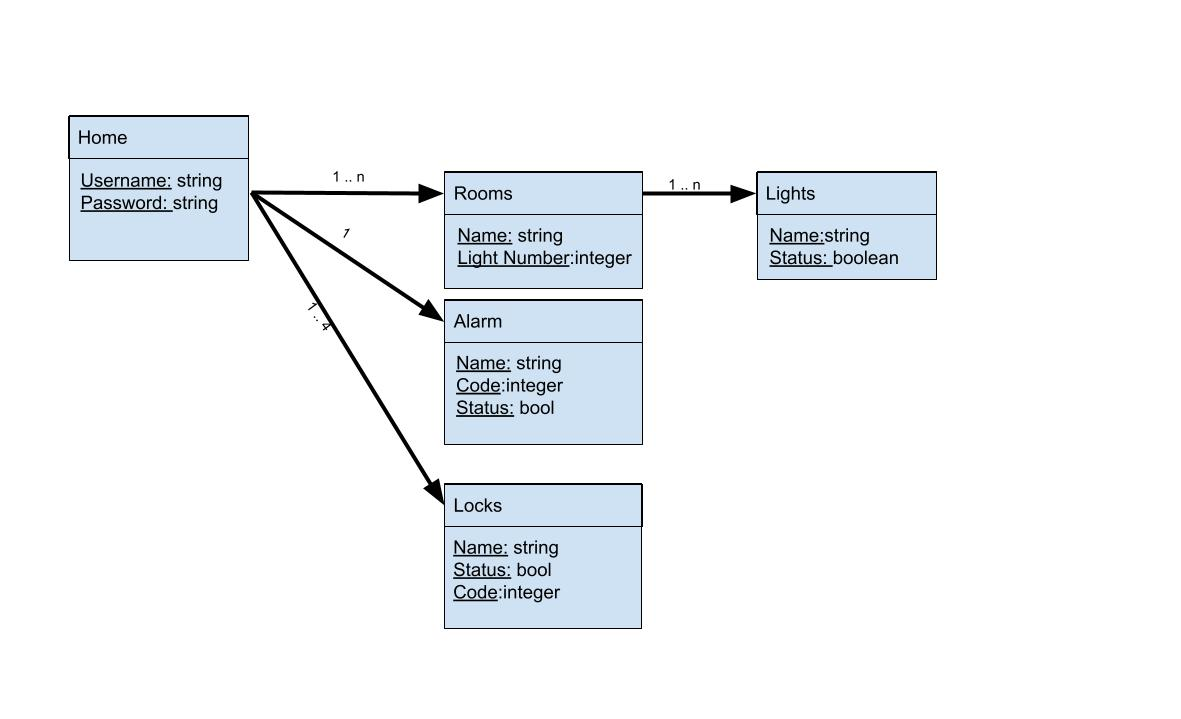
\includegraphics[scale=0.5]{data_model}
				\caption{Data models follow the specifications}
				\label{fig:datamodel}
			\end{figure}
		This is the simplest data model which we can use as a template given the fact that as we move one with this project we are going to be adding more features such as setting RGB colors,change lock combinations, setting the brightness, and later on be able to add more devices
		\subsection{Business Logic}
			\subsubsection{Basic Operations}
				\begin{itemize}
					\item Login/Logout
					\item Check Status of each device
					\item Change Status of each devices
				\end{itemize}
			\subsubsection{Storyboard}
				\begin{figure}[H]
					\centering
					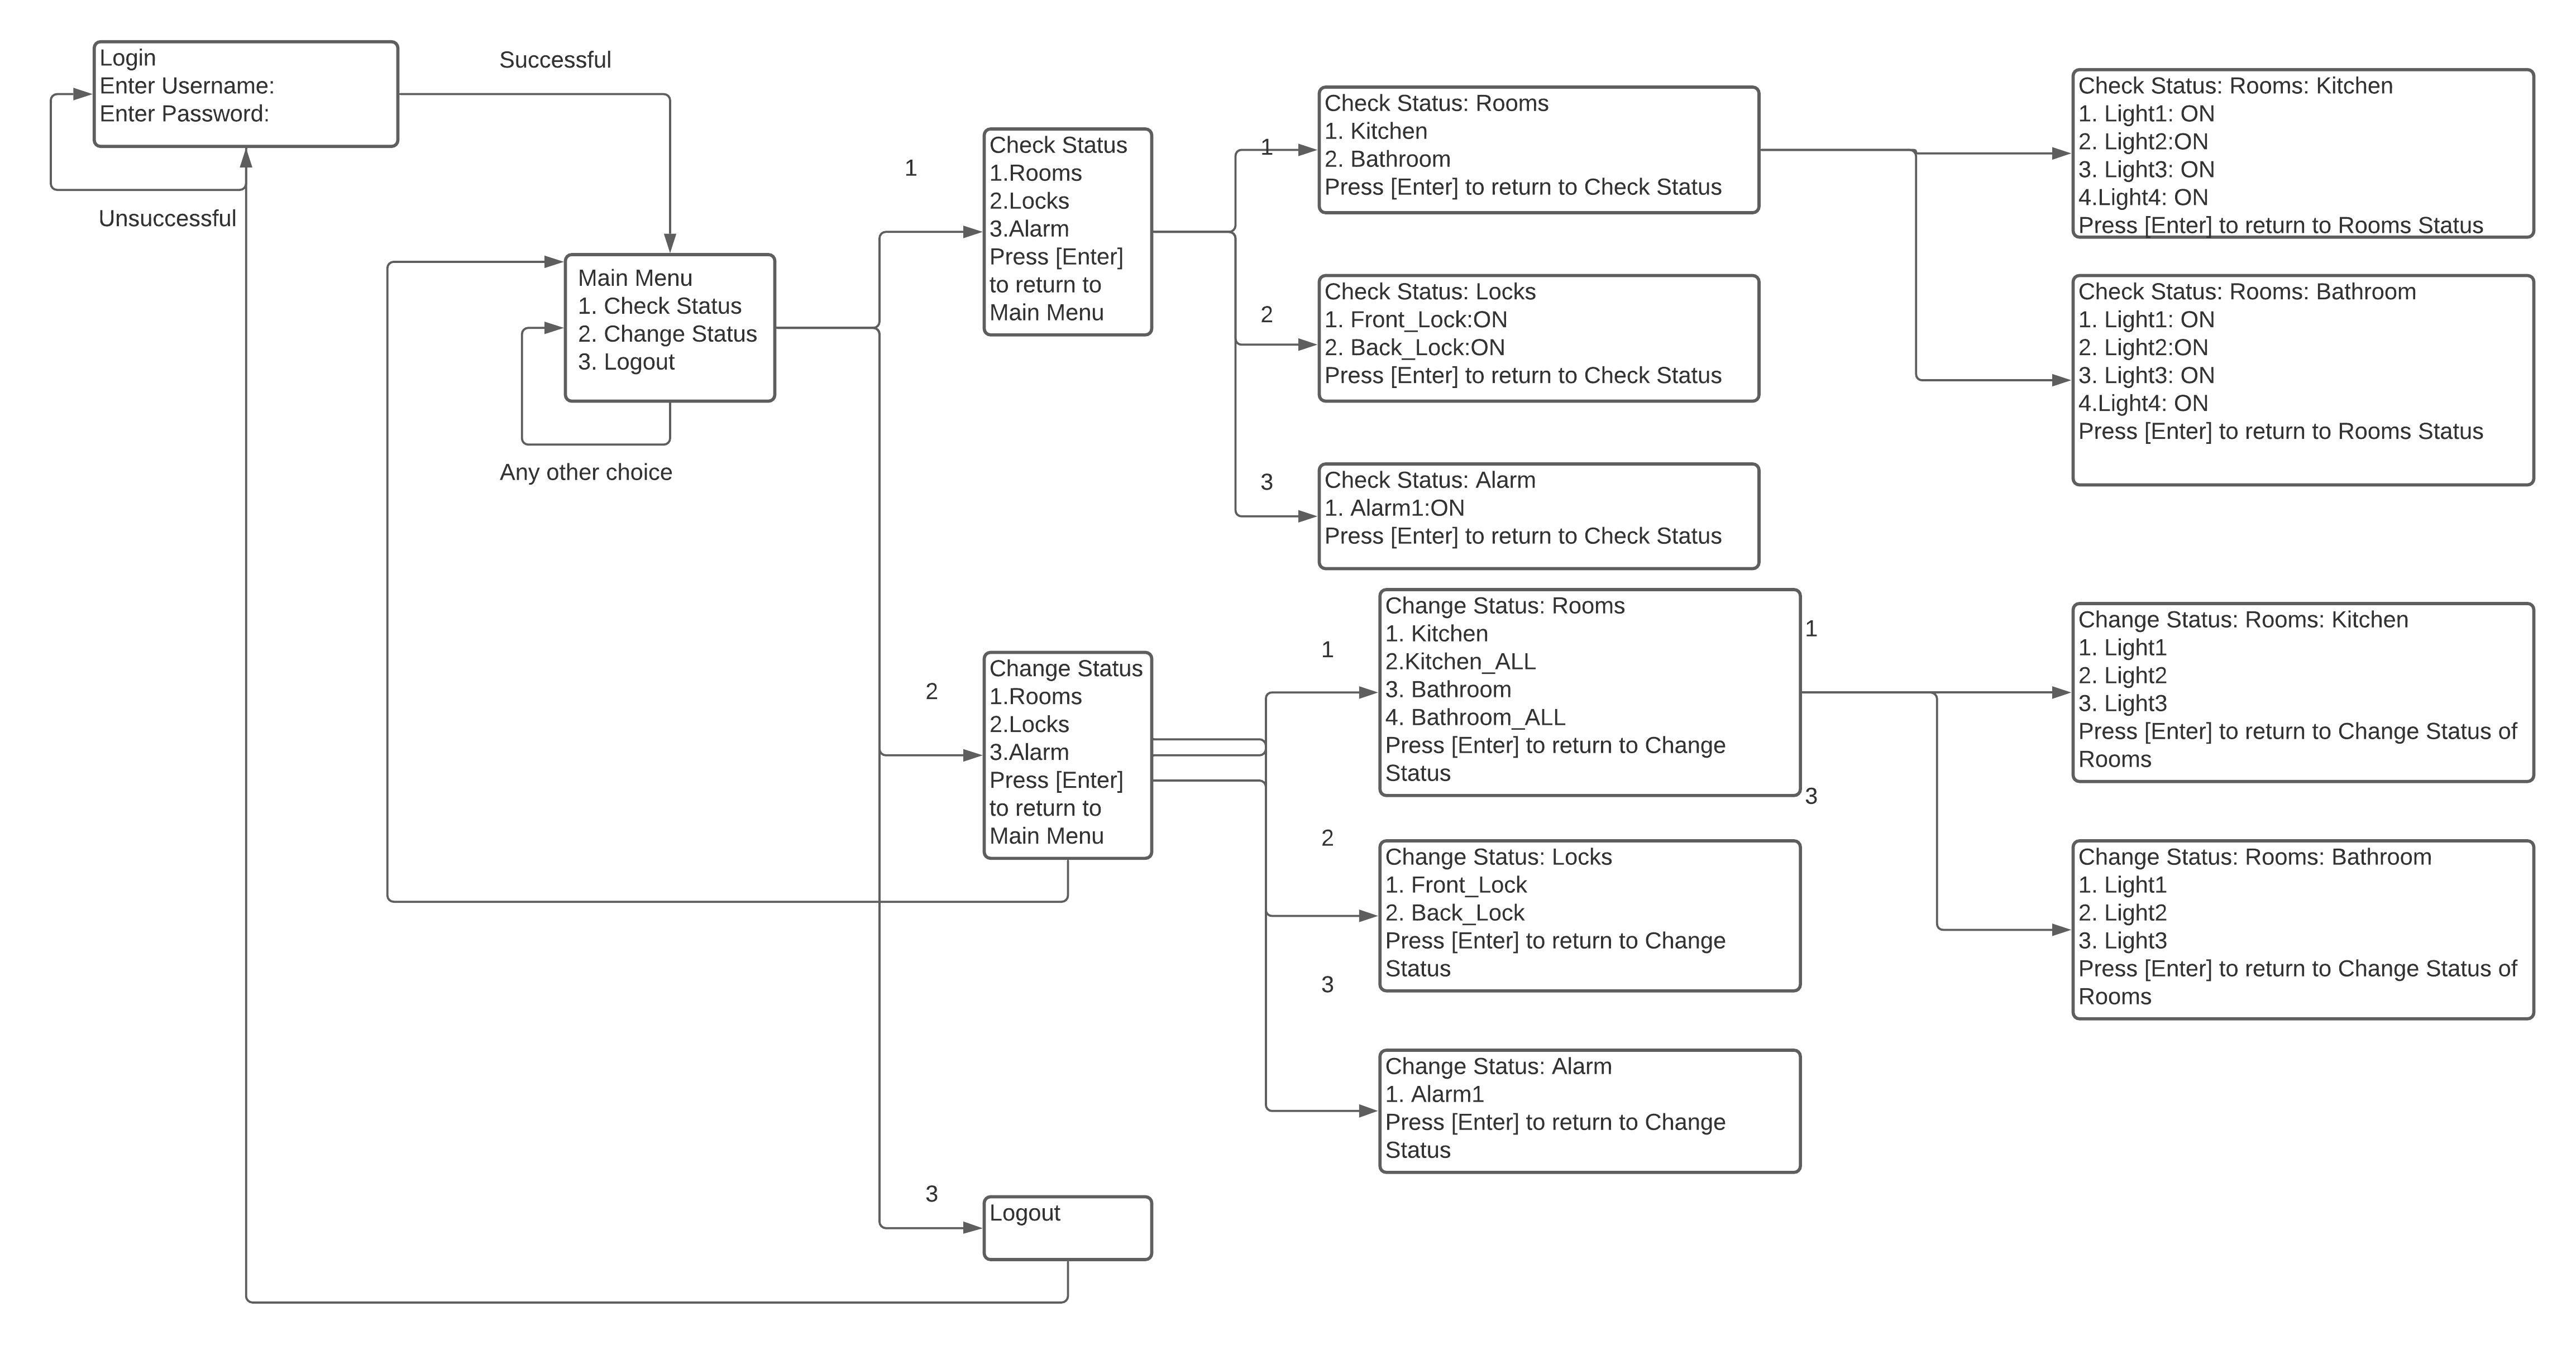
\includegraphics[scale=0.5]{StoryBoard}
					\caption{}
					\label{fig:storyboard}
				\end{figure}
			The reason I chose to divide my check status and change status  based on devices is because that is the method that my google home uses show the status of my devices and change the status of my devices. In my opinion the most effective method is by simply having a single main menu with a all the options since it leads to less amount of packets being transferred back and forth between the client and the server and can therefore reduce bandwidth.
			As we move on, I am going to implement more menus for the alarm,locks, and lights as way to provide more features for each device
		\subsection{Sever state chart}
			\begin{figure}[H]
				\centering
				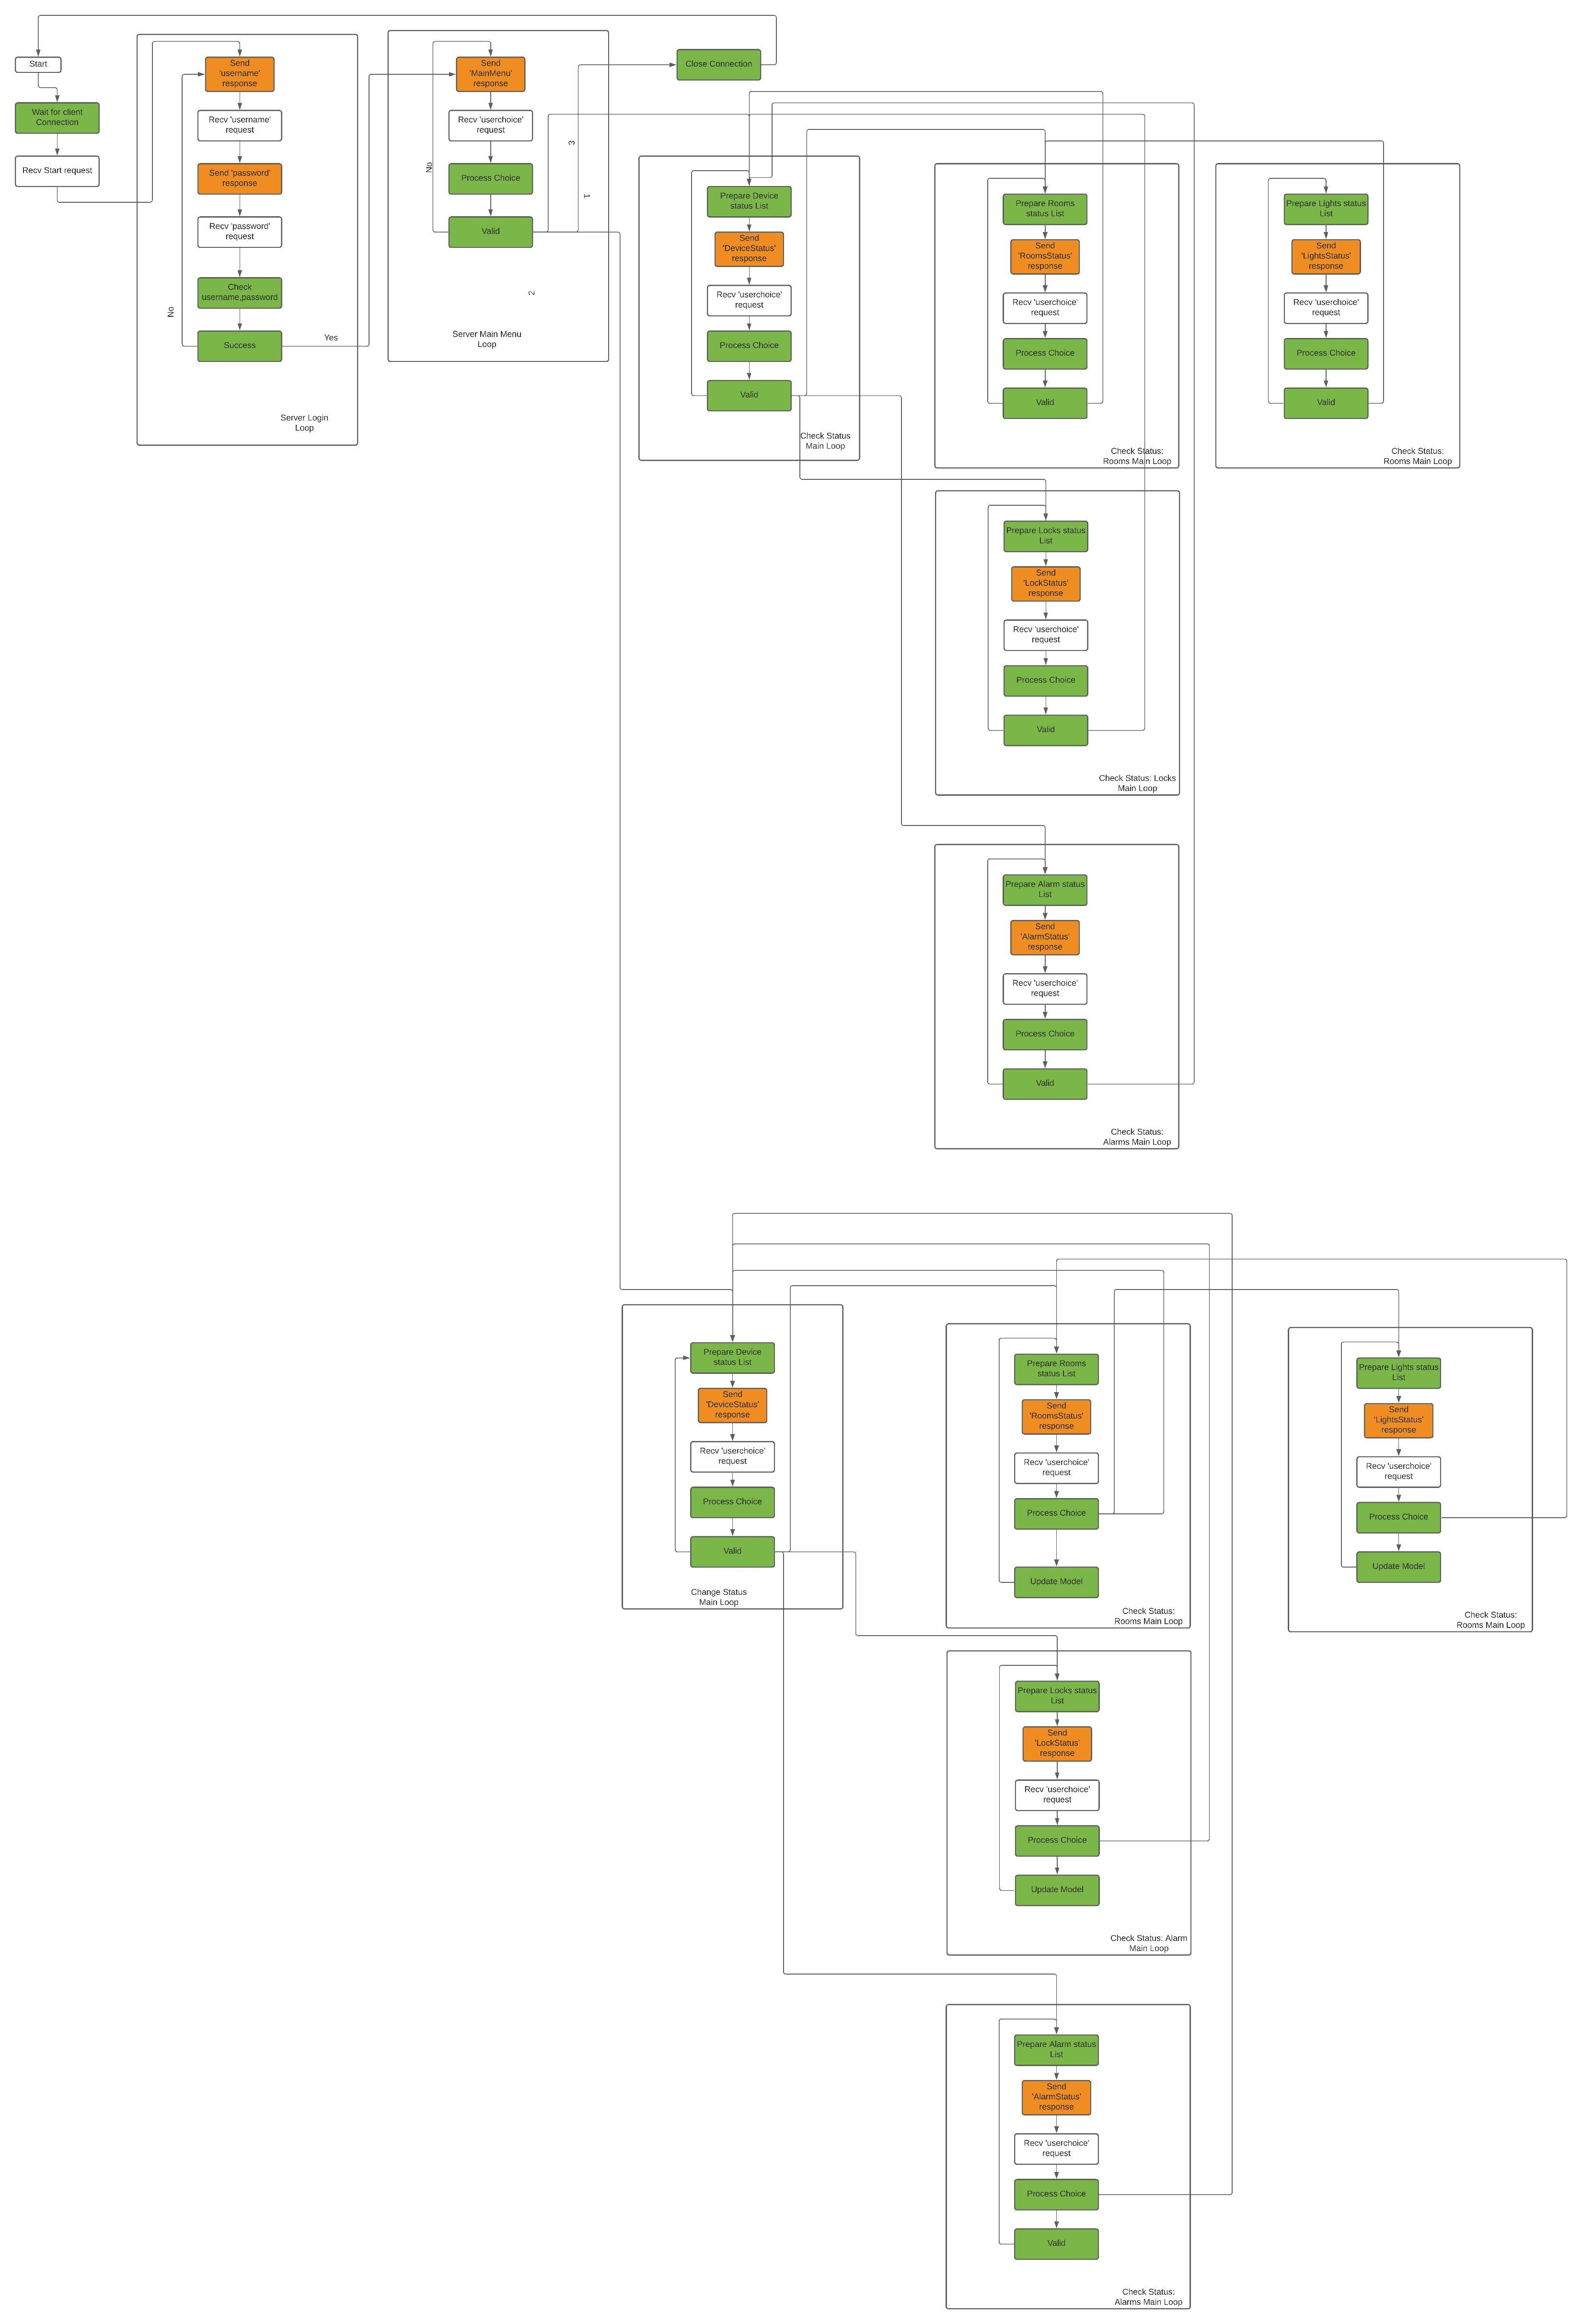
\includegraphics[scale=0.5]{server_state_diagram}
				\label{fig:serverstatediagram}
			\end{figure}
		The server state diagram starts by simply waiting for the client to establish a connection. After establishing a connection, the user is going to be asked to send their username and password which is going to be check by the server based on the data model. If the username and password is correct then we move on to the main menu else we return back to the server login menu. After entering the main menu, the user needs to send the server a request for either checking status of a device, changing the status of a device, or logging out . After the user request the either check or change the status, they are going to receive the list of devices available to choose from. After requesting a device, the user is going to either the rooms, locks, or alarms available to them so they can either change or check the status. For changing the status there is an extra step in which the server updates the data model for each change and returns back to displaying the status of that device. For each menu there is always a return option which is simply by requesting to press enter. 
		\subsection{Client State Chart}
			\begin{figure}[H]
				\centering
				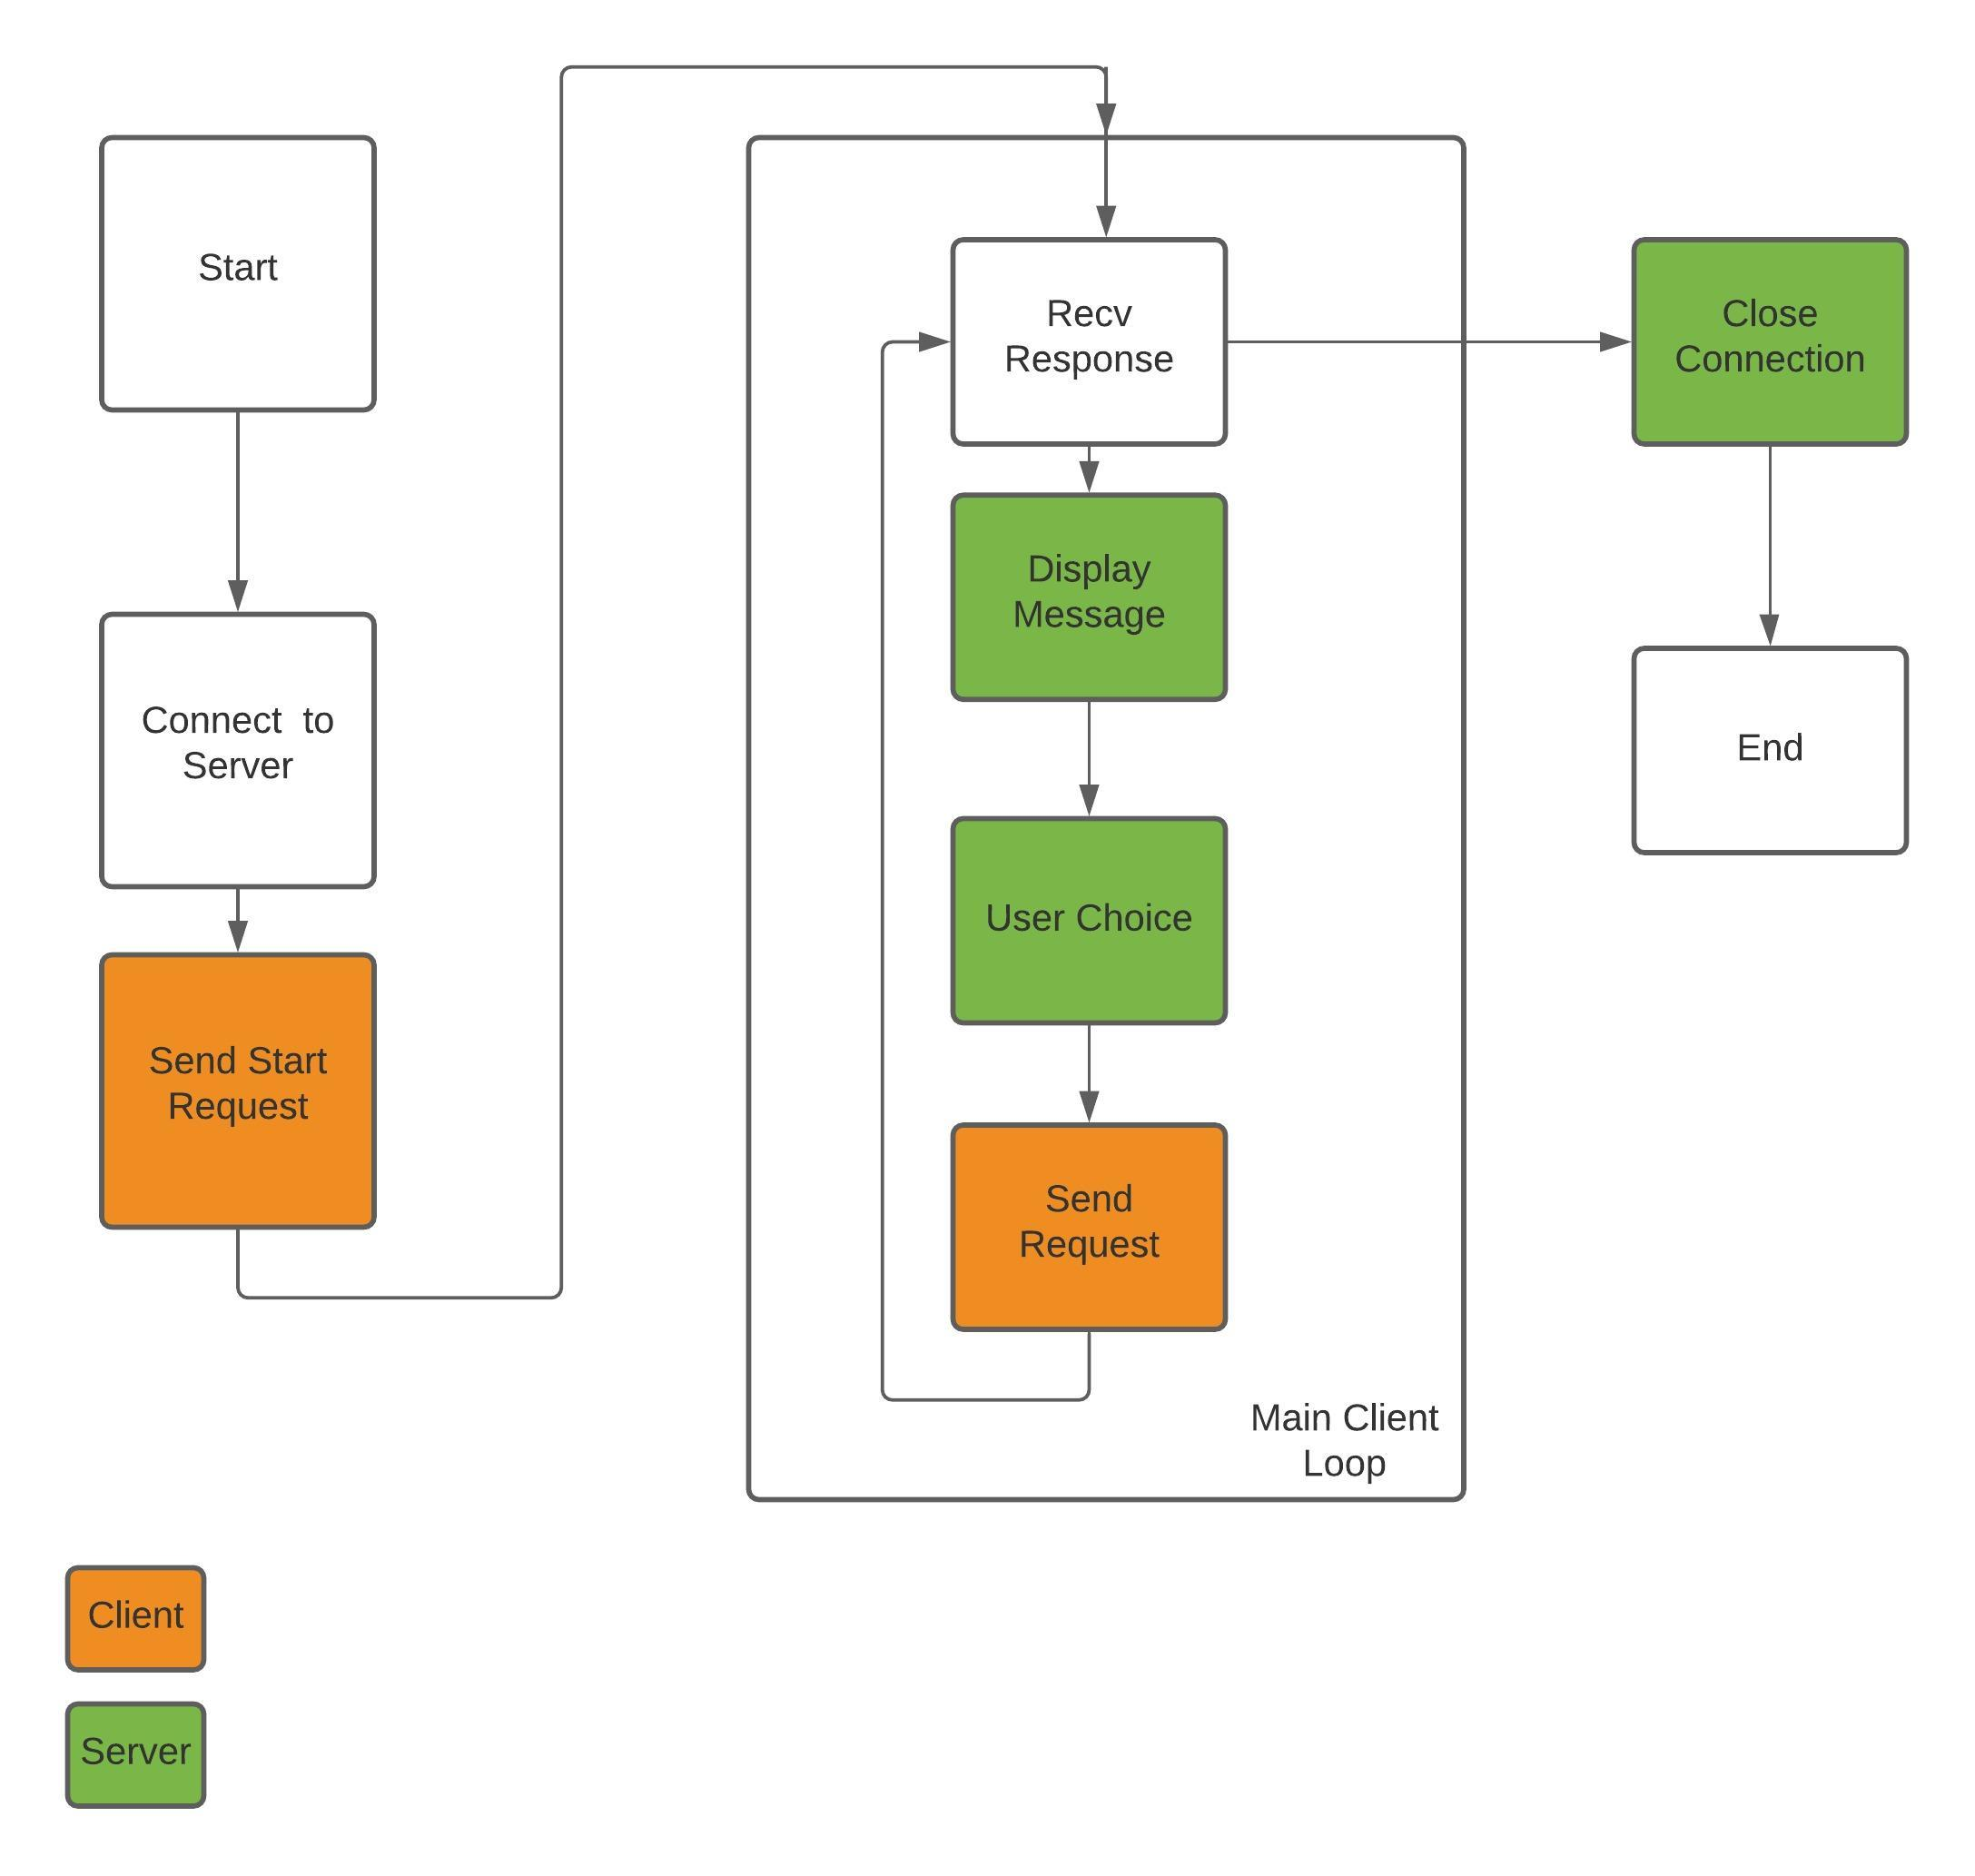
\includegraphics[scale=0.5]{Client_State_Diagram}
				\label{fig:clientstatediagram}
			\end{figure}
		The client state diagram starts by simply establishing a connection between the server and the client. Then the server sends the client a message,which the user uses to make a request. After the request is sent to the server, the server makes a decision based on that request and executes a command. The connection between the server and the client ends when the user decides to log out.
		\subsection{Application Protocol Design}
			\begin{table}[H]
				\centering
				\resizebox{\textwidth}{!}{%
					\begin{tabular}{llll}
						\hline
						\multicolumn{1}{|l|}{Client Application Protocols} & \multicolumn{1}{l|}{Parameters}                 & \multicolumn{1}{l|}{Body}    & \multicolumn{1}{l|}{Description}                                                                            \\ \hline
						\multicolumn{1}{|l|}{START}                        & \multicolumn{1}{l|}{none}                       & \multicolumn{1}{l|}{none}    & \multicolumn{1}{l|}{Establishes connection with the server}                                                 \\ \hline
						\multicolumn{1}{|l|}{CHOICE}                       & \multicolumn{1}{l|}{Lines=24 character,lines=0} & \multicolumn{1}{l|}{None}    & \multicolumn{1}{l|}{Based on the options of the server, the user can send up to 24 character to the server} \\ \hline
						\multicolumn{1}{|l|}{END}                          & \multicolumn{1}{l|}{None}                       & \multicolumn{1}{l|}{none}    & \multicolumn{1}{l|}{Ends the connection between the client and the server}                                  \\ \hline
						&                                                 &                              &                                                                                                             \\
						&                                                 &                              &                                                                                                             \\
						&                                                 &                              &                                                                                                             \\ \hline
						\multicolumn{1}{|l|}{Server Application Protocols} & \multicolumn{1}{l|}{Parameters}                 & \multicolumn{1}{l|}{Body}    & \multicolumn{1}{l|}{Description}                                                                            \\ \hline
						\multicolumn{1}{|l|}{USER}                         & \multicolumn{1}{l|}{Lines=24 character}         & \multicolumn{1}{l|}{Line}    & \multicolumn{1}{l|}{Ask the user for the username}                                                          \\ \hline
						\multicolumn{1}{|l|}{PASS}                         & \multicolumn{1}{l|}{Line=24 character}          & \multicolumn{1}{l|}{Line}    & \multicolumn{1}{l|}{Ask the user for the password}                                                          \\ \hline
						\multicolumn{1}{|l|}{LIST}                         & \multicolumn{1}{l|}{Line=24 character}          & \multicolumn{1}{l|}{Line(s)} & \multicolumn{1}{l|}{Gives the user options which they can chose from}                                       \\ \hline
						\multicolumn{1}{|l|}{ERROR}                        & \multicolumn{1}{l|}{Line=24 character}          & \multicolumn{1}{l|}{Line(s)} & \multicolumn{1}{l|}{Send the user information about an error in the system and waits for his choice}        \\ \hline
						\multicolumn{1}{|l|}{END}                          & \multicolumn{1}{l|}{None}                       & \multicolumn{1}{l|}{None}    & \multicolumn{1}{l|}{The server ends the connection between the client and the server}                       \\ \hline
					\end{tabular}
				}
			\end{table}
	\section{Example}
		\begin{figure}[H]
			\centering
			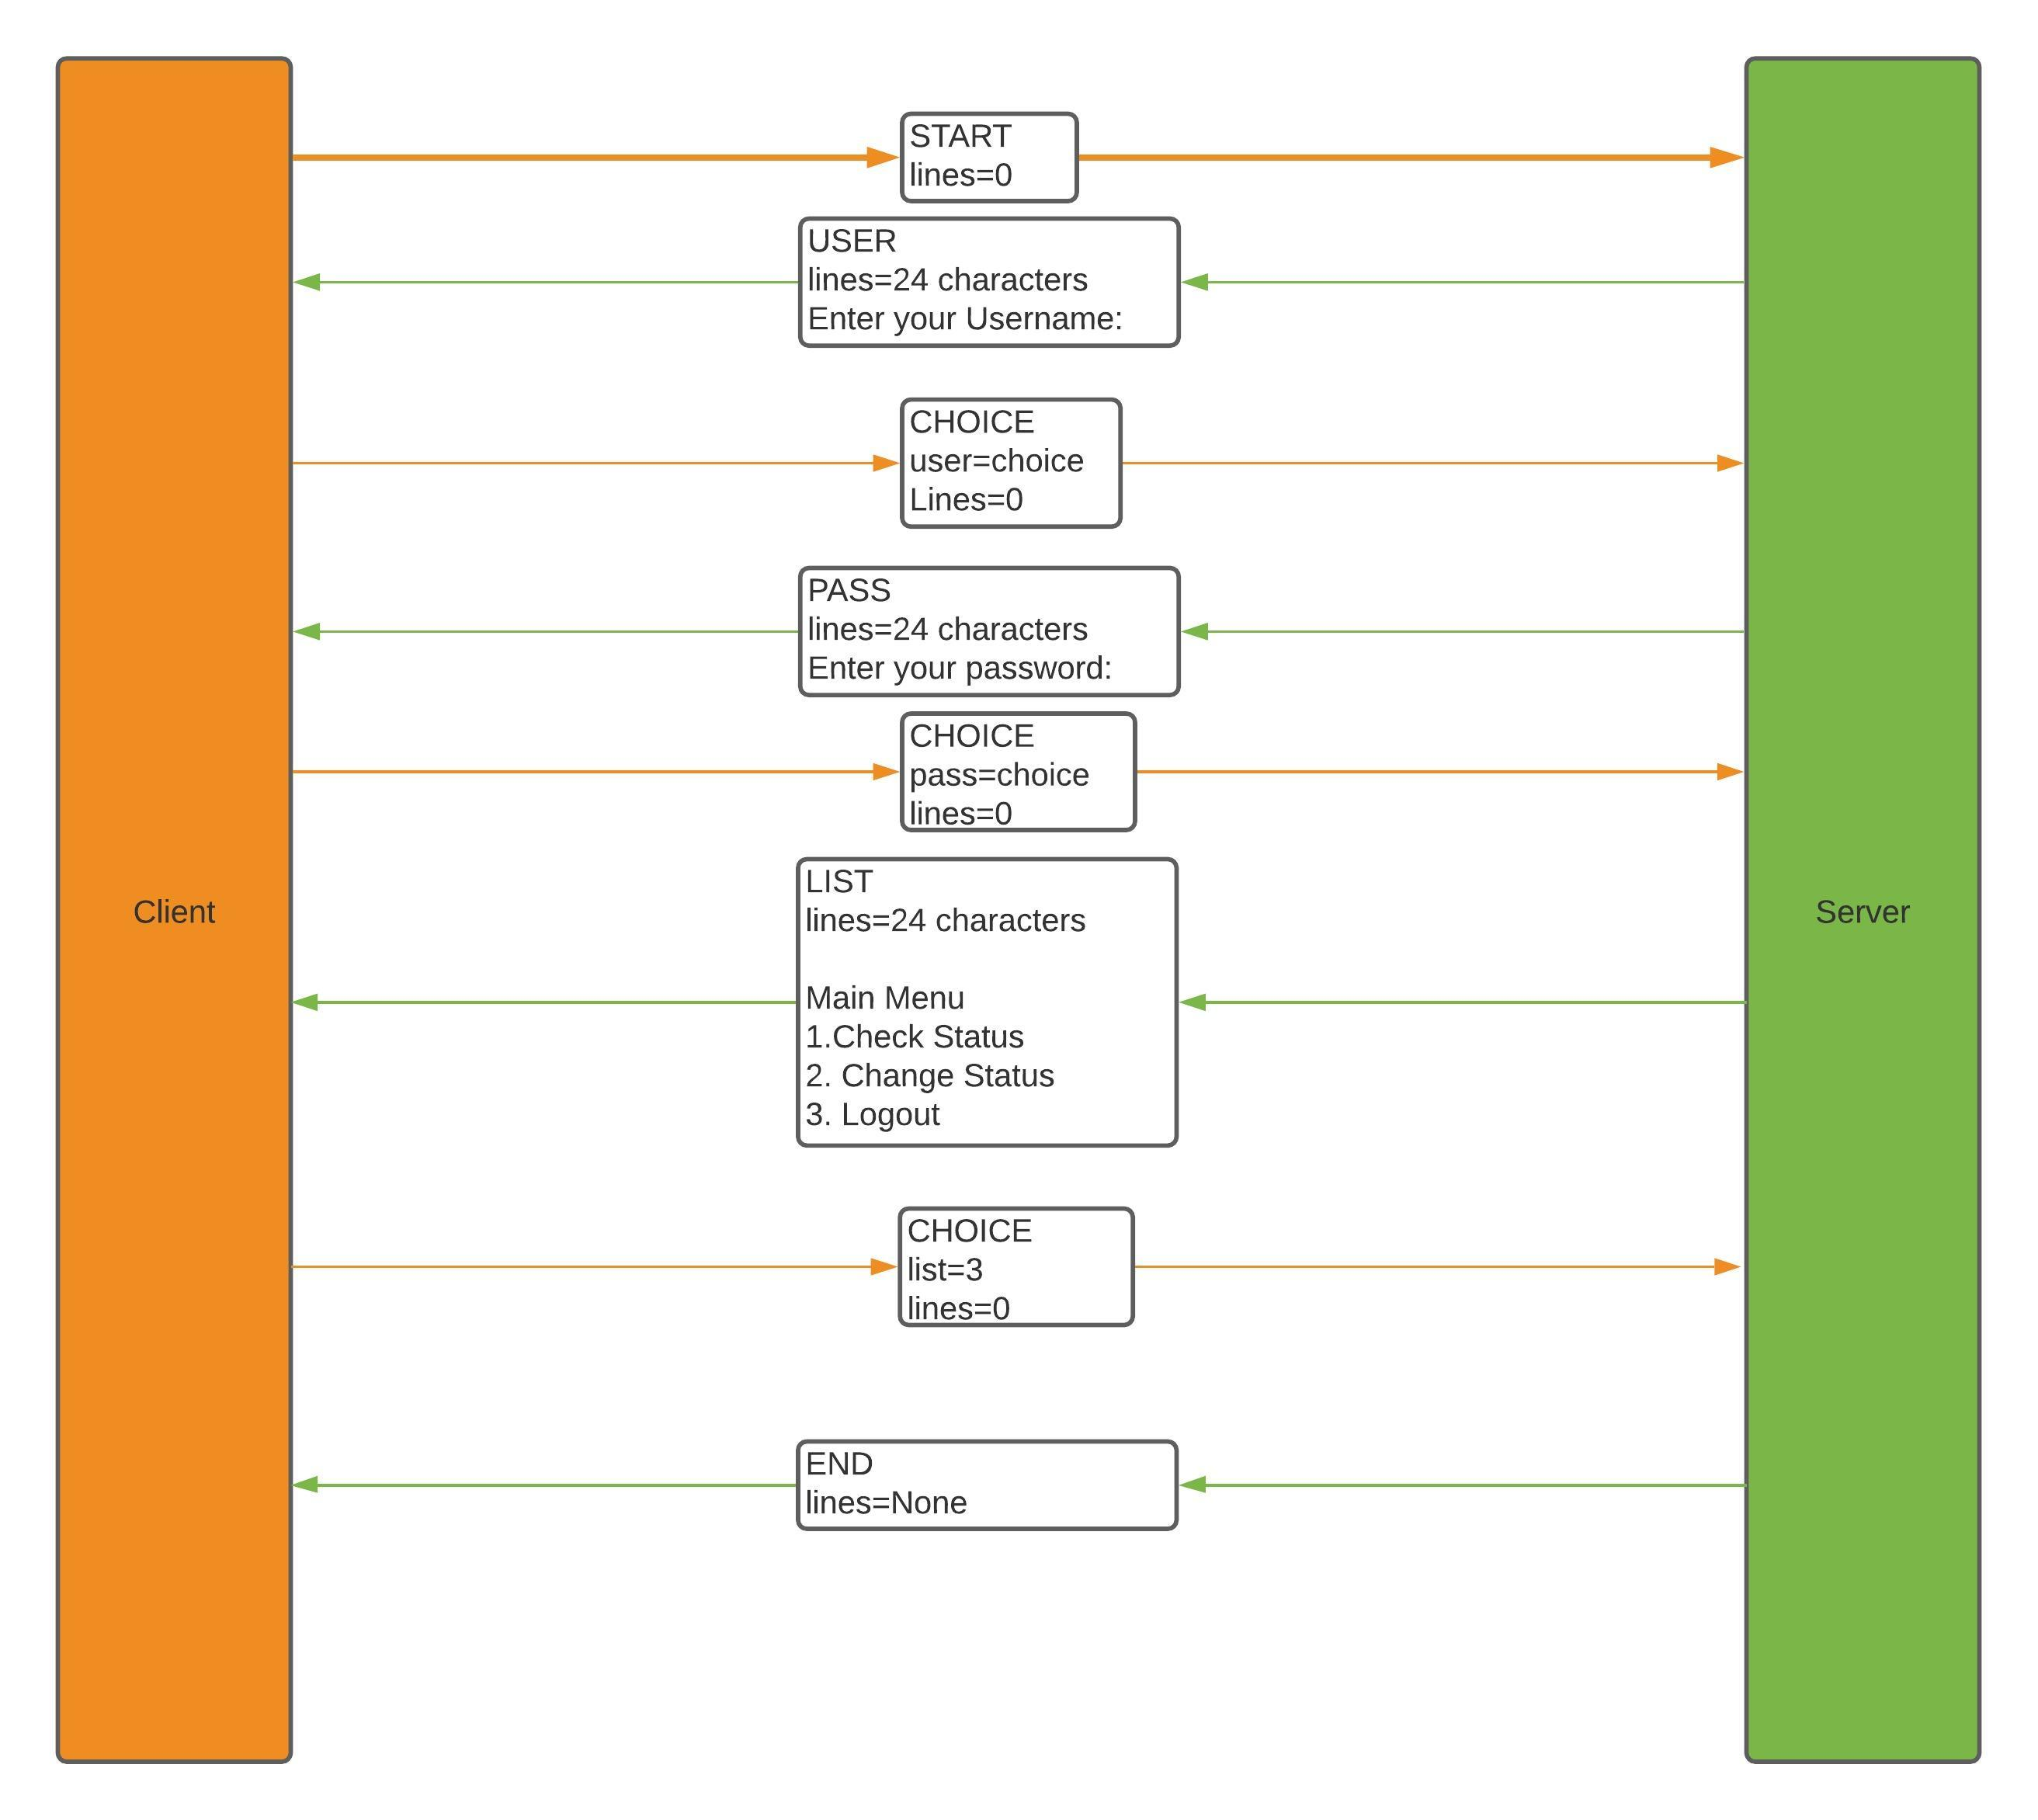
\includegraphics[scale=0.5]{Examples}
			\label{fig:examples}
		\end{figure}
	\section{Data model}
			\begin{lstlisting}
				#ifndef _DATAMODEL_H_
				#define _DATAMODEL_H
				#include <iostream>
				#include <string>
				#include <vector>
				using namespace std;
				
				class light
				{
				public:
				string name;
				bool status;
				};
				
				
				
				class room
				{
				public:
				vector<light> l;
				};
				
				
				
				class rooms
				{
				public:
				vector<room> r;
				string name;
				int light_number;
				};
				
				
				class alarm
				{
				public:
				string name;
				int code;
				};
				
				
				
				class lock
				{
				public:
				string name;
				int code;
				};
				
				
				
				class locks
				{
				public:
				vector<lock> llock;
				};
				
				
				class home
				{
				private:
				string password;
				string username;
				public:
				rooms n;
				alarm a;
				locks lo;
				void setUsername(string newUsername);
				void setPassword(string password);
				};
				#endif
			\end{lstlisting}
		\section{Message Protocol}
			\subsection{Client}
				\subsubsection{Header file}
					\begin{lstlisting}
						#ifndef _CLIENT_MARSHAL_H_
						#define _CLIENT_MARSHAL_H_
						#include <iostream>
						#include <string>
						#include <stdio.h>
						#include <stdlib.h>
						#include <sstream>
						#include <vector>
						using namespace std;
						class server_message
						{
						public:
						string options;
						string message;
						vector<string> lines;
						int num_lines;
						void printing()
						{
						cout<<options<<"    "<<num_lines<<"     "<<message<<endl;
						for(unsigned int i=0;i<lines.size();i++)
						{
						cout<<lines[i]<<endl;
						}
						
						}
						};
						
						class client_message
						{
						public:
						string options;
						int decision;
						void printing()
						{
						cout<<options<<"    "<<decision;
						}
						};
						
						server_message unmarshal(string message)
						{
						string command;
						server_message res;
						stringstream ss(message);
						ss>>command;
						if(command=="USER")
						{   res.options="USER";
						getline(ss,res.message);
						}
						else if(command=="PASS")
						{
						res.options="PASS";
						getline(ss,res.message);
						}
						else if(command=="LIST")
						{
						res.options="LIST";
						getline(ss,res.message,'\\');
						ss>>res.num_lines;
						vector<stringstream> tt(res.num_lines);
						string temp;
						int i=0;
						while(ss>>temp)
						{
						if(res.message=="\\\\")
						{
						break;
						}
						else if(temp=="\\")
						{
						i++;
						}
						else
						{
						tt[i]<<temp<<" ";
						}
						}
						for(unsigned int j=0;j<tt.size();j++)
						{
						string temp2;
						getline(tt[j],temp2);
						res.lines.push_back(temp2);
						}
						}
						else if(command=="ERROR")
						{
						res.options="ERROR";
						getline(ss,res.message);
						ss>>res.message;
						}
						else if(command=="END")
						{
						res.options="END";
						getline(ss,res.message);
						ss>>res.message;
						}
						else
						{
						}
						return res;
						}
						
						
						string marshal(client_message cm)
						{
						stringstream ss;
						string result;
						if(cm.options=="START")
						{
						ss<<cm.options<<" "<<cm.decision;
						}
						else if(cm.options=="CHOICE")
						{
						ss<<cm.options<<" "<<cm.decision;
						}
						else if(cm.options=="END")
						{
						ss<<cm.options<<" "<<cm.decision;
						}
						else if(cm.options=="ERROR")
						{
						ss<<cm.options<<" "<<cm.decision;
						}
						else
						{
						} 
						getline(ss,result);
						return result;
						}
						#endif
					\end{lstlisting}
				\subsubsection{Test File}
					\begin{lstlisting}
						#include <iostream>
						#include <string>
						#include <stdio.h>
						#include <stdlib.h>
						#include <sstream>
						#include "client_marshal.h"
						using namespace std;
						int main(int argc,char*argv[])
						{
						if(argc==2)
						{
						cout<<"Testing unmarshal"<<endl;
						server_message test1;
						test1 =unmarshal(argv[1]);
						test1.printing();
						}
						
						if(argc>2)
						{
						cout<<"Testing Marshall"<<endl;
						client_message test;
						test.decision=atoi(argv[2]);
						test.options=argv[1];
						cout<<marshal(test)<<endl;
						}
						return 0;
						}
					\end{lstlisting}
				\subsubsection{Makefile}
					\begin{lstlisting}
						all:client server_marshal.h client_marshal.h
						echo Testing the client
						client:client.cpp client_marshal.h
						g++ client.cpp -o client				
						test_client: client client.cpp client_marshal.h
						@./client "USER Enter Your Username:"
						@./client "PASS Enter your Password:"
						@./client "ERROR There is an Error:"
						@./client "END Ending the Connection"
						@./client "LIST Here are the options: \ 1 1.Option 1 \\"
						@./client "LIST Here are the options: \ 2 1.Option 1 \ 2. Option 2 \\"
						@./client "LIST Here are the options: \ 3 1.Option 1 \ 2. Option 2 \ 3. Option 3 \\"
						@./client "LIST Here are the options: \ 4 1.Option 1 \ 2. Option 2 \ 3. Option 3 \ 4. Option 4 \\"
						@ echo
						@ echo
						@./client "START" "1"
						@./client "CHOICE" "1"
						@./client "END" "1"
						@./client "ERROR" "1"
						clean:
						rm client
					\end{lstlisting}
				\subsection{Results}	
					\begin{figure}[H]
						\centering
						\includegraphics[scale=0.5]{"../../../../../../../Pictures/Screenshot from 2021-03-02 21-02-45"}
						\caption{Results for the client marshalling}
						\label{fig:screenshot-from-2021-03-02-21-02-45}
					\end{figure}
		\section{Server Marshal}
			\subsection{Header File}
			\subsection{Test program}
			\subsection{Makefile}
				
\end{document}